Scintillators are materials widely employed for radiation detection in nuclear physics. Scintillators convert kinetic energy of the incoming particles into light which can be detected and quantified. Light emission is produced due to the photon de-excitation of atoms of fluorescent molecules in the material.

Light production is linear with energy for a wide energy range of incoming particles. Scintillators should have good optical properties, such as being transparent to the wavelength of their own emission and having a refractive index close to that of photosensor windows in order to optimize optical coupling and light transmission. Photon emission in scintillators is a statistical process that follows a Poisson distribution.

Scintillators can be organic or inorganic. Inorganic scintillators normally have a high atomic number and density, so their light output is high. For these reasons they are suitable for gamma-ray spectroscopy. Organic scintillators are generally fast and they are used for charged particles and neutron detection. This section is focussed on organic scintillators since they are the ones used in the TRITIUM detector. Organic scintillators are based on fluorescent molecules dissolved in a base solvent, usually aromatic hydrocarbons as $\ce{C_{18}H_{14}}$, $\ce{C_{24}H_{22}N_{2}O}$ or $\ce{C_{15}H_{11}NO}$ with an average atomic number between 3.5 and 5. The fluorescent molecules of organic scintillators have a $\pi$-electron structure. The energy levels of their electrons are commonly illustrated with a Jablonsky diagram, shown in Figure \ref{fig:JablonskyDiagram}. This diagram shows the fundamental singlet states, $S_{0i}$, the excited singlet states, $S_{jk}$, and the excited triplet states, $T_{lm}$. The energy difference between $S_1$ and $S_0$ states is around $3$ to $4~\eV$, which corresponds to the visible photon emission. As shown in the figure, each energy state is split into close sublevels separated around $0.15~\eV$. This fine energy structure is due to excitations of molecular vibrational modes tagged by the second index of the energy states. As the energy levels and sublevels have an energy larger than the thermal energy, $0.025~\eV$, electrons are in the ground state $S_{00}$ at STP. When a particle deposits its kinetic energy in a scintillator, the valence electrons are excited very fast ($\tau \approx 1~\pico\second$) to higher singlet energy states and are quickly de-excited to the first singlet excited state, $S_{10}$, through non-radiative processes known as internal conversion. These electrons can de-excite to the fundamental singlet state, $S_{00}$, through three different physical mechanisms:

\begin{figure}[htbp]
\centering
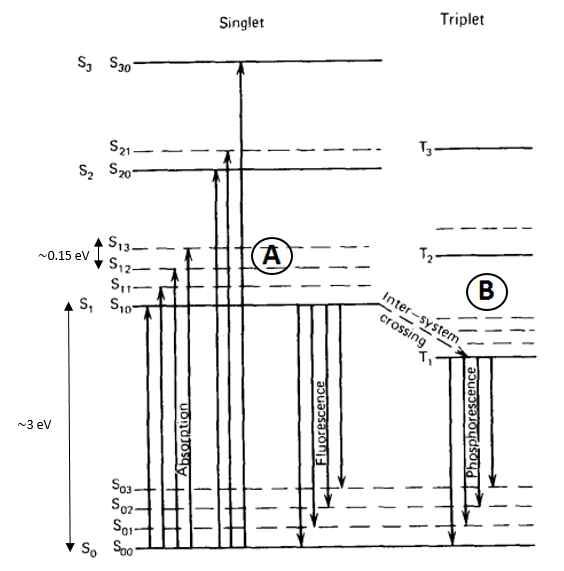
\includegraphics[scale=0.57]{3DesignPrinciples/32Tritium_detector/JablonskyDiagram.png}
\caption{Jablonsky diagram\label{fig:JablonskyDiagram}~\cite{Knoll}.}
\end{figure}

\begin{enumerate}

\item{} Prompt fluorescence (process A in Figure \ref{fig:JablonskyDiagram}), where the electron in the $S_{10}$ level  is de-excited to a sublevel of the ground state $S_{0i}$, emitting a photon. This process happens immediately after the excitation of the scintillator molecules (of the order of nanoseconds after excitation). Each scintillator has a characteristic emission spectrum. Organic scintillators are practically transparent to their own fluorescense emission because scintillating photons have less energy than the excitation energy. This effect is called Stokes shift and it is represented in Figure \ref{fig:StokesShift}. The intensity of the fluorescence emission in an organic scintillator versus time is the combination of two exponential functions, one associated with the lifetime of the level $\tau$ (of the order of nanoseconds), and the other associated with the energy level population $\tau_1$ (of the order of picoseconds) \cite{Knoll},

\begin{equation}
I=I_0\left(e^{-t/\tau} - e^{-t/\tau_1}\right) 
\label{eq:IntensityTimeScintillator}
\end{equation}

\begin{figure}[htbp]
\centering
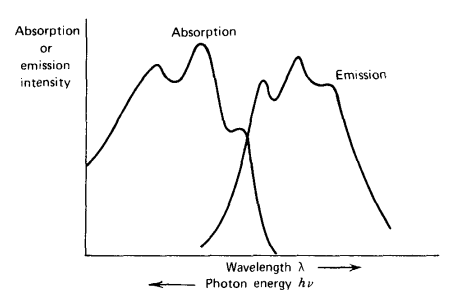
\includegraphics[scale=0.7]{3DesignPrinciples/32Tritium_detector/StokesShift.png}
\caption{Stokes shift\label{fig:StokesShift}~\cite{Knoll}.}
\end{figure}

\item{} Phosphorescence, where the electron that is in the first singlet excited state crosses to a triplet excited state (process B in Figure \ref{fig:JablonskyDiagram}). Such a transition process is called "intersystem crossing". The triplet state is a metastable state with a longer lifetime than fluorescence, of the order of milliseconds after scintillator excitation.

\item{} Delayed fluorescence, which occurs when an electron is in a triplet excited state but its transition to the ground state is forbidden. In this case, the electron interacts with another electron in a similar state, falling to the first singlet state and quickly de-exciting to the ground state, 

\begin{equation}
T_{1} ~+~ T_{1}~ \longrightarrow ~ S_{1} ~+~ S_{0} ~+~ phonons
\label{eq:DelayFluorescence}
\end{equation}

This emission has the same emission spectrum as the prompt fluorescence, but with a longer lifetime.
\end{enumerate}
As the prompt fluorescence light produces the scintillator signal, the detector design should optimize its collection and detection and reduce other possible physical mechanisms like phosphorescence or delayed fluorescence. One of the most important parameters that characterizes the scintillator is the scintillation yield, defined as the number of photons emitted per unit of absorbed energy. This yield depends on the type of particle and on other mechanisms that do not produce prompt fluorescence light, like phosphorescence, delayed fluorescence, and non radiative processes like internal conversion. The scintillator yield is normally quoted by the manufacturer for mips\footnote{A mip or minimum ionizing particle is a particle that has a speed at which the ionization produced is minimal.}.
